% ---------------------------------------------------------------------
% Cloned from the HES-SO//Master canvas 2019
% ---------------------------------------------------------------------


\chapter{Experiments \& Results}
\label{chap:experiments-results}
Intending to get a hold on the Word2Vec technology and as a complement to the analysis chapter \ref{chap:analysis}, the following are the experiments made during the \gls{dp} and their results.

\section{Build a Word2Vec model}
\paragraph{Getting started with Word2Vec}
As recommended to the author, this section has been made following the Gensim tutorial by Machine Learning Plus \cite{article:gensim-tutorial}. There is not much to say about this section except that the author, with its current Word2Vec knowledge, would recommend this tutorial to anyone willing to get started with Word2Vec. \\

As overviewed in the tutorial mentioned above, using pre-trained models is good to get started quickly, and building a model on a small dataset is fair enough to get for various tasks; however, in the case of this \gls{dp}, the author wanted to understand how everything works behind the scene.

\subsection{Build the Vocabulary}
The first step is to build a Word2Vec model is to build its vocabulary. Luckily, it is straight forward, as it does not require much tweaking. Indeed, it is only required to decide if the lemmatization will be present if stop words are included, if there is word frequency threshold, and if the symbols such as punctuation are used.\\

For the \gls{dp}, two dictionaries were built, both with default settings from the WikiCorpus method but differentiated by the presence or not of the lemmatization. This function is from the Gensim package corpora.wikicorpus and is specialized for Wikipedia dump. The following is the function definition \cite{article:gensim-api}:

%[language=Python]
\begin{lstlisting}
gensim.corpora.wikicorpus.WikiCorpus(
        fname, processes=None, lemmatize=True,
        dictionary=None, filter_namespaces=('0', ),
        tokenizer_func=<function tokenize>,
        article_min_tokens=50, token_min_len=2,
        token_max_len=15, lower=True, 
        filter_articles=None)
\end{lstlisting}

\paragraph{Notebook in Appendices}
\begin{itemize}
    \setlength\itemsep{0em}
    \item pa-build-dictionary
\end{itemize}


\subsection{Build the Wikipedia Model}
This section could resume about half of the \gls{dp}, which in theory should not be too difficult; however, hours passed at a high rate to finally being able to produce Wikipedia models easily. The following is the function definition \cite{article:gensim-api}: \\

\begin{lstlisting}
gensim.models.word2vec.Word2Vec(sentences=None,
        corpus_file=None, size=100, alpha=0.025,
        window=5, min_count=5, max_vocab_size=None,
        sample=0.001, seed=1, workers=3,
        min_alpha=0.0001, sg=0, hs=0, negative=5,
        ns_exponent=0.75, cbow_mean=1,
        hashfxn=<built-in function hash>, iter=5,
        null_word=0, trim_rule=None, sorted_vocab=1,
        batch_words=10000, compute_loss=False,
        callbacks=(), max_final_vocab=None)
\end{lstlisting}

\paragraph{Notebook in Appendices}
\begin{itemize}
    \setlength\itemsep{0em}
    \item pa-w2v-mono-training
\end{itemize}


\subsection{Split and Retrain Technic}
\label{experiment:split-retrain}
During the initial phases of the \gls{dp}, the English Wikipedia Dump was too large for the machine available to the author. [\ref{experiment:environments}] As a result, it was required to find a workaround to make it work anyway.

\paragraph{First step}
Split the Wikipedia corpora into chunks.

\paragraph{Second step}
Retrain [\ref{analyse:retrain}] the model on each chunks.

\paragraph{Notebooks in Appendices}
\begin{itemize}
    \setlength\itemsep{0em}
    \item pa-wikidump-splitter
    \item pa-build-word2vec-on-splits
\end{itemize}

\subsubsection{Issue}
\label{experiment:split-retrain-issue}
Sadly, it was found out later, while using the CPU Dedicated Server [\ref{experiment:cpu-monster}], that the vocabulary was not updated, resulting in a model containing only the initial chunk vocabulary. Even if the limited vocabulary represents well the whole contexts from the English Wikipedia, it does not make much sense as a whole.\\

Due to the original purpose to fix specific hardware limitation [\ref{experiment:icolab}], the solution was discontinued as the limitations were solved with new hardware. If the code must be reused, the vocabulary should be updated at each chunk iteration.


\section{Environments}
\label{experiment:environments}
The language used during the whole chapter is Python with the Gensim framework and Jupyter Notebook. The main dataset for the experiment is the English Wikipedia Dump from 09th May 2019 [\ref{sota:datasets}].

\subsection{Local Machines}
\label{experiment:local-machines}
At the beginning of the project, it was suggested to the author that his local machines would be enough to use Word2Vec; however, even after various tweaking, it concluded that the hardware on author's local machines was limited. Indeed, the RAM, CPU, and Disk Space were not enough to handle the English Wikipedia dump dataset (bzip2: 16Gb, raw: 90Gb) [\ref{experiment:memory-issues}]. 

\subsubsection{Macbook Pro Specifications}
\begin{itemize}
    \setlength\itemsep{0em}
    \item CPU: 2.3GHz Intel Core i7, 4 cores
    \item RAM: 16GB 1600MHz DDR3
\end{itemize}

\subsubsection{Windows Specifications}
\begin{itemize}
    \setlength\itemsep{0em}
    \item CPU: 2.50GHz Intel Xeon E5-2680 v3
    \item RAM: 12GB 2400MHz DDR4 
\end{itemize}

\subsection{iColab GPU Server}
\label{experiment:icolab}
As a solution, the iCoSys Institut at HES-SO//Fribourg provided access to a remote machine dedicated to \gls{dl} student projects. This infrastructure could hold the first experiments; however, due to the nature of the server, the Word2Vec training was highly impacted for the large Wikipedia dataset. Indeed, the server was build for GPU usage instead of CPU intensive computation, in addition to the RAM being shared across all users, the author was not able to train the full model in one shot, and had to use a custom made data splitter with a retraining [\ref{analyse:retrain}] workaround to make it work [\ref{experiment:split-retrain}].\\

However, even with the used workaround, the time to train the whole dataset took 3 days and 20 hours, and sadly for what was discovered afterward, an incomplete model [\ref{experiment:split-retrain-issue}].

\subsubsection{iColab GPU Server Specification}
\begin{itemize}
    \setlength\itemsep{0em}
    \item CPU: 2.10GHz Intel Xeon E5-2620 v4
    \item RAM: 128GB
\end{itemize}


\subsection{\gls{aws}}
\label{experiment:aws}
With the hope to solve the author's local machines [\ref{experiment:local-machines}] limitations and to decrease drastically the time spent on the iColab GPU Server [\ref{experiment:icolab}], the author tried deploying a virtual machine on the \gls{aws} EC2 service\cite{article:aws-ec2-dl-install}.\\

The outcome was not satisfying at all. Indeed, the author's account at \gls{aws} is restricted from powerful machines \cite{article:aws-ec2-service-limits}. Indeed, useful machines for the project with a high amount of RAM and CPUs were not available to use. \\

However, for the sake of the experiment, the author tried the largest machine available to him, the c4.8xlarge \cite{article:aws-ec2-pricing}. Except for being expensive; the results were not as good as it should have been expected: indeed the performance was similar to the iColab GPU Server.

\subsubsection{c4.8xlarge}
\begin{itemize}
    \setlength\itemsep{0em}
    \item vCPU: 64
    \item ECU: 132
    \item RAM: 60 GB
    \item Price: 1.591 per Hour
\end{itemize}


\subsection{Microsoft Azure Notebook}
\label{experiment:azure-notebook}
Desperate to train the wikipedia model, the author also tried the Azure Notebook service\cite{article:azure-notebook}. The results are similary limited as for \gls{aws} [\ref{experiment:aws}],.


\subsection{Google Colab}
\label{experiment:google-colab}
Even the Google Colab server, which is meant for GPU and TPU processing was tested \cite{article:google-colab}. Even by taking care of keeping the session alive which implies bypass an inactivity timeout after 90 minutes\cite{article:google-colab-timeout}, the maximum lifetime per instance of 12 hours \cite{article:google-colab-faqs} and RAM limitation made it impossible to accomplish the training.


\subsection{CPU Dedicated Server}
\label{experiment:cpu-monster}
After insisting, a dedicated server with enough CPU and RAM from the iCoSys Institut was provided to the author.\\

It has become the machine of reference for all the results for the \gls{dp}.

\subsubsection{CPU Monster Specification}
\begin{itemize}
    \setlength\itemsep{0em}
    \item CPU: 8x 1.2Ghz AMD Opteron 6176
    \item RAM: 192GB DIMM
\end{itemize}


\subsection{Memory Issues}
\label{experiment:memory-issues}
The main issue encountered with the machines was the memory allocation. Indeed, the whole dataset is loaded into the RAM and that the multi-core merging function is using temporary additional RAM [\ref{fig:error-memory-allocation}].\\

\paragraph{Dataset}
English Wikipedia Dump is weighting 16Gb in its compressed bzip2 form, and about 90Gb in its raw form.\\

\paragraph{Local machine [\ref{experiment:local-machines}]}
The problem is clearly coming from the RAM available, 12GB and 16GB.

\paragraph{iColab [\ref{experiment:icolab}]}
Even if the RAM is in theory enough for the dataset, it seems that the limitation comes from the server configuration; indeed, the RAM is shared across all users and is probably limited.

\paragraph{AWS [\ref{experiment:aws}]}

\paragraph{Azure Notebook [\ref{experiment:azure-notebook}]}
Free azure notebook is limiting the at 4GB per session.

\paragraph{Google Colab [\ref{experiment:google-colab}]}
As an honorable mention, the ram is limit to 13GB per session.

\begin{figure}[ht!]
\centering
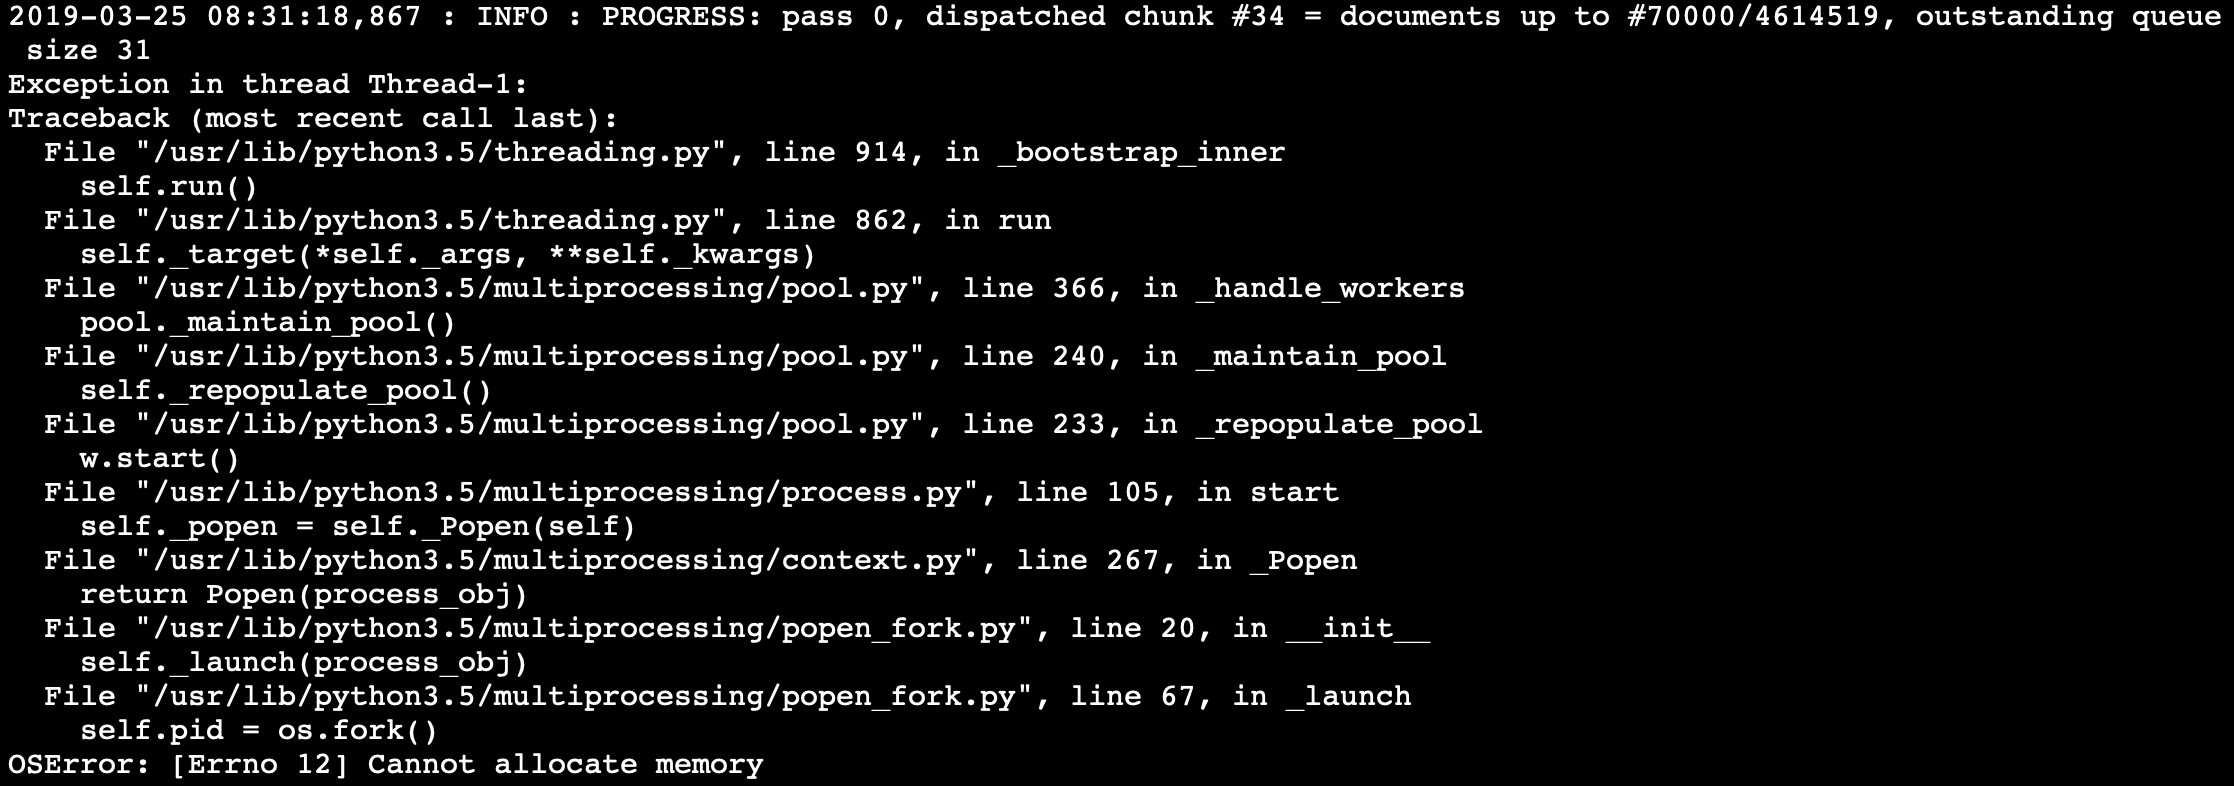
\includegraphics[width=\linewidth]{99-imgs/gensim_memory_allocation_error}
\caption{Memory Allocation Error}
\label{fig:error-memory-allocation}
\end{figure}


\section{Play with Word2Vec}
The second most time consuming and informative part of the \gls{dp} is when the author could finally play with the Word2Vec model.

\subsection{Common Word2Vec Operations}
As seen in the analysis chapter, the common operations such as Geometrical Vector Operations [\ref{analyse:geometric-operations}], Similarities [\ref{analyse:common-tasks}], Analogies [\ref{analyse:analogies}] and Normalization [\ref{analyse:normalization}] were played with on the large wikipedia model.

\paragraph{Notebooks in Appendices}
\begin{itemize}
    \setlength\itemsep{0em}
    \item pa-play-with-w2v-enwiki-lemmatized.ipynb
    \item a-play-with-w2v-enwiki-unlemmatized.ipynb
\end{itemize}

\subsection{Models Diversity and Time Benchmarks}
To profit the most from the CPU Dedicated Server, and as building Wikipedia models are time-consuming, the author started a process of keeping the machine busy by producing Word2Vec models with different parameters based on the Wikipedia dump. All the following parameters were altered:

\begin{itemize}
    \setlength\itemsep{0em}
    \item \gls{cbow} \ref{analyse:cbow}
    \item Skip-Grams \ref{analyse:skip-grams}
    \item Lemmatization \ref{analyse:lemmatization}
    \item Dimensions \ref{analyse:dimensions}
    \item Window \ref{analyse:window}
    \item Epochs \ref{analyse:epochs}
\end{itemize}

\paragraph{Spreadsheet in Appendices}
\begin{itemize}
    \setlength\itemsep{0em}
    \item pa-models-created-and-time-benchmarks
\end{itemize}


\subsection{Visual Representation}
To get a hold on what a Word2Vec model is, the author implemented a visual representation of the multi-dimensional space using the T-SNE \cite{article:tsne} technic, which flatters high dimensional points into a two-dimensional space. For example, the top 100 similar vectors to the word \textit{Woman} on the figure \ref{fig:tsne-top100-woman}.

\paragraph{Notebook in Appendices}
\begin{itemize}
    \setlength\itemsep{0em}
    \item pa-w2v-explore-models
\end{itemize}

\begin{figure}[h!]
    \centering
    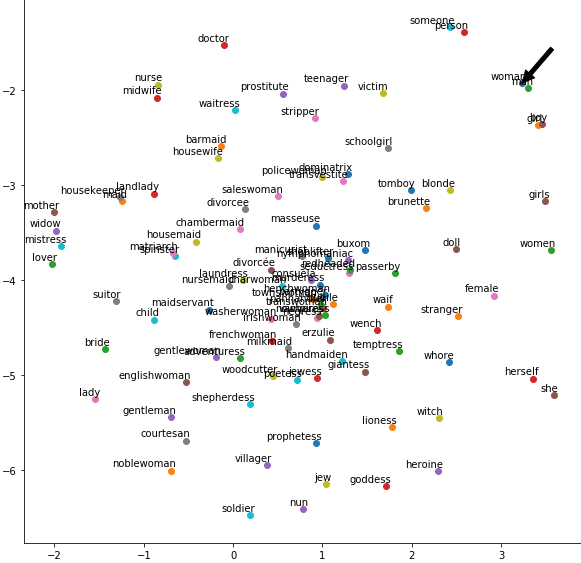
\includegraphics[width=\textwidth,keepaspectratio=true]{tsne-top100-woman}
    \caption{Top 100 T-SNE representation of similar words vectors to Woman}
    \label{fig:tsne-top100-woman}
\end{figure}


\subsection{Word Vector Influences}
To pursue the understanding of how vectors are interacting with each other, the author implemented a solution that applies an arbitrary value to each element of a word vectors and evaluates the impact of this change on the word similarities. For example, for the word vector \textit{Federer}, the top 5 similar words will be tracked while each element of the Federer vector will be alternated elements. As a way to keep track of the altered element on the visual representation, each vector has been labeled with its altered index as seen in figure \ref{fig:word-influence}. 

\paragraph{Notebook in Appendices}
\begin{itemize}
    \setlength\itemsep{0em}
    \item pa-w2v-explore-vector-influence
\end{itemize}

\begin{figure}[h!]
    \centering
    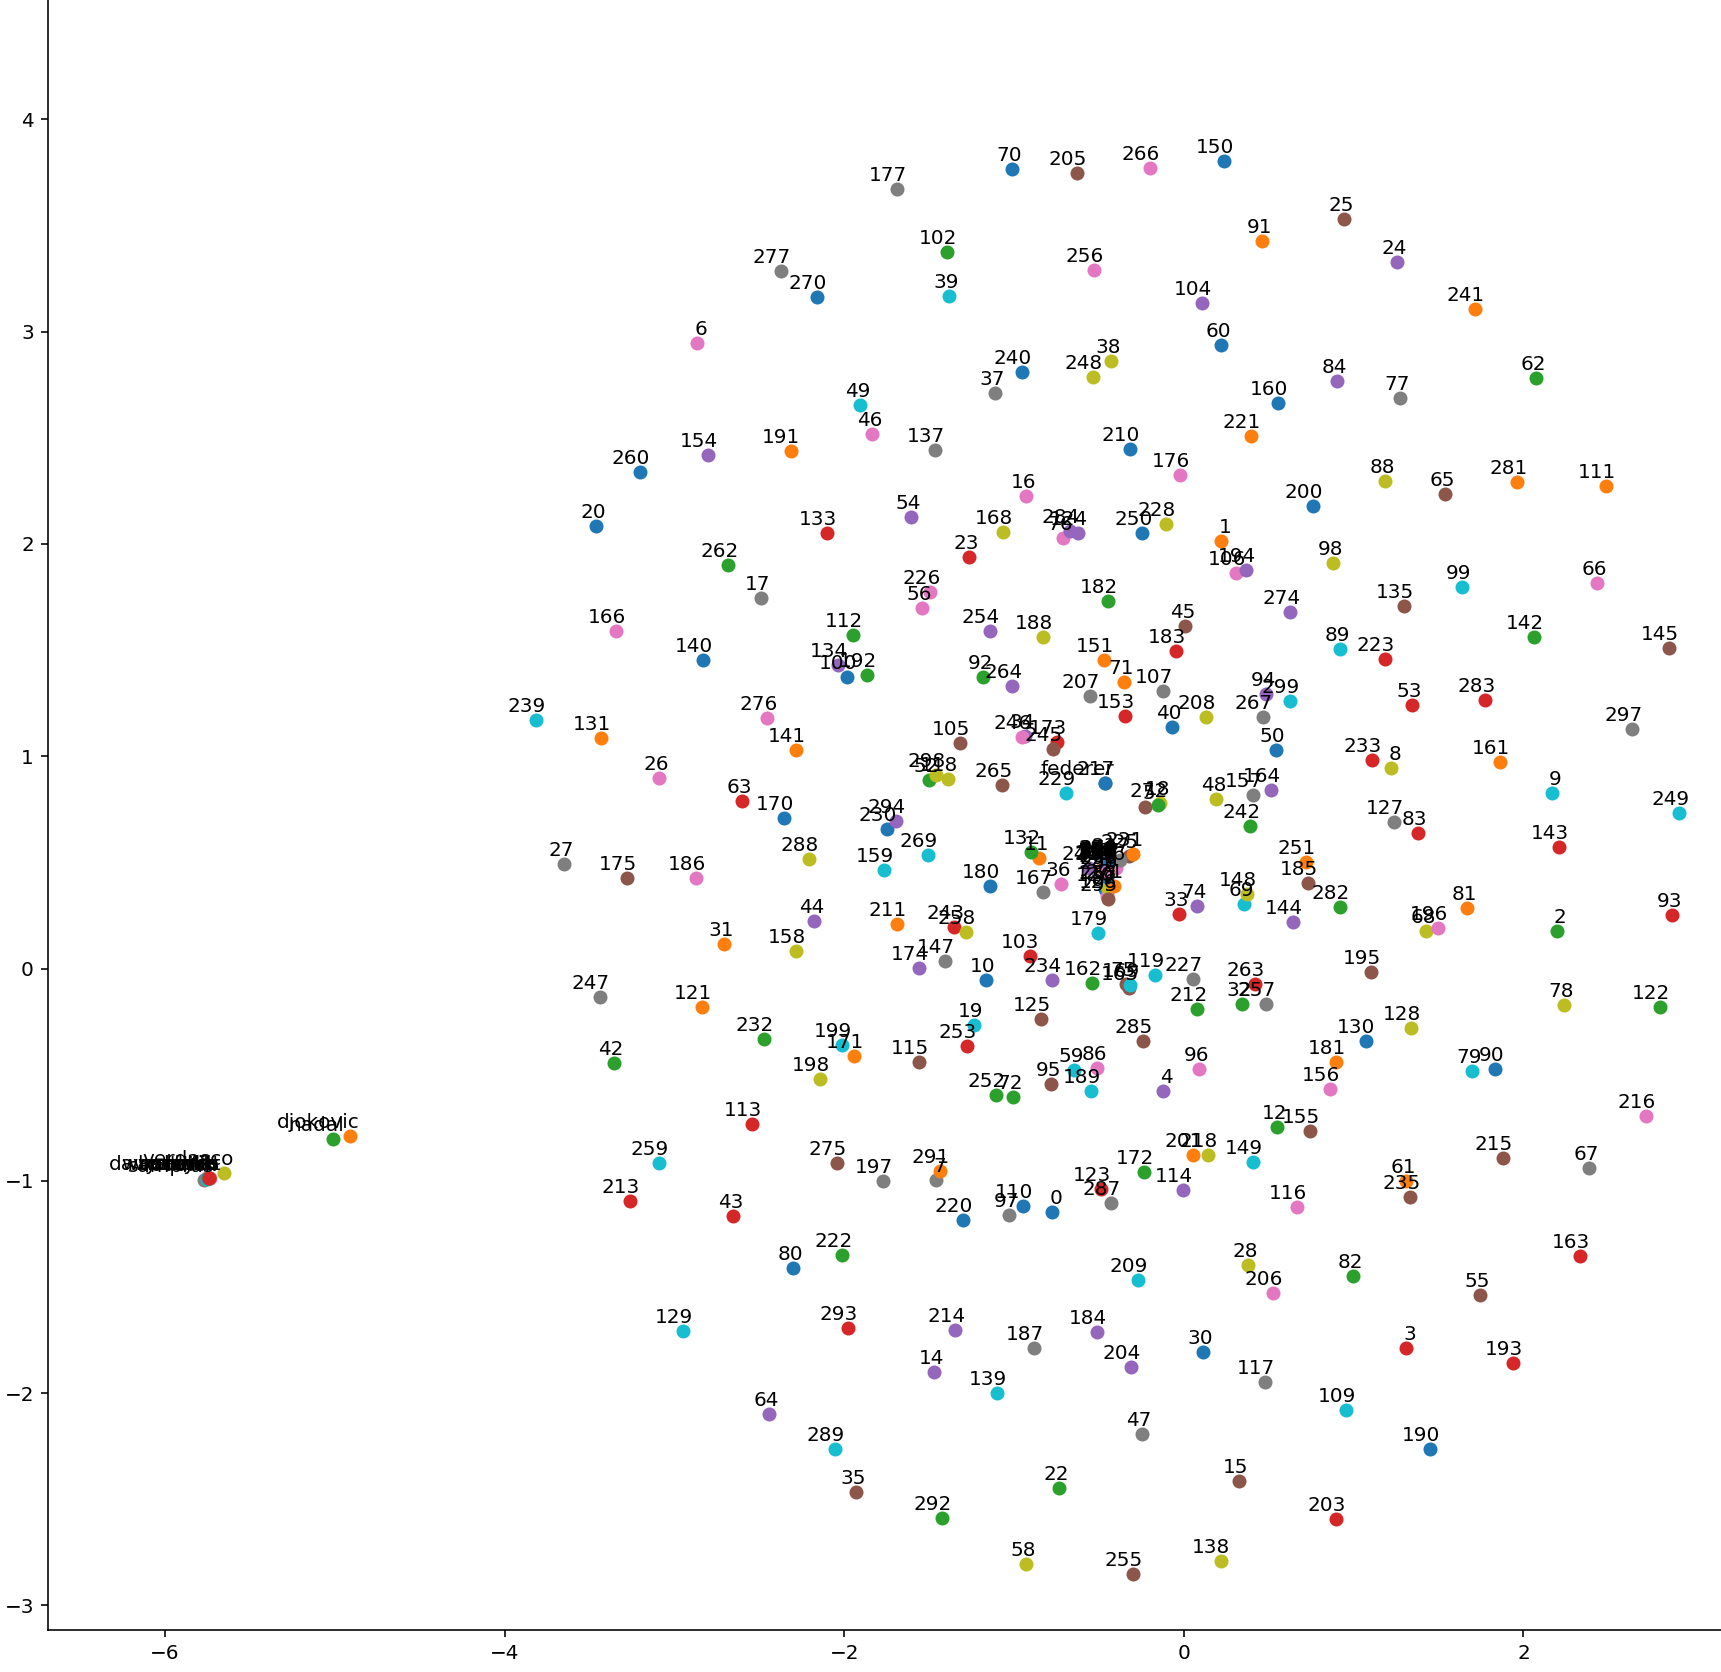
\includegraphics[width=\textwidth,keepaspectratio=true]{word-influence}
    \caption{Top 5 T-SNE of similar words vectors to the word Federer with altered vector elements}
    \label{fig:word-influence}
\end{figure}


\section{Proactivity}
As part of the \gls{dp} red line [\ref{questions:redline}], it was asked to explore the Word2Vec possibilities to make chatbots proactive.

\subsection{Sentence Generator}
To explore the possibilities of proactivity, the author tried to used geometric operations [\ref{analyse:geometric-operations}] to generate sentences. Various vector manipulations were used to alternate and generate new sentences out of \textit{Proverbs} and \textit{Facts}, such as word additions, arbitrary value subtractions, and even the use of random vectors. \\

The idea was that, to make a chatbot proactive, it needs to be able to generate sentences out of a meaningful context. Moreover, a solution was to make a sentence generator of facts, based on real proverbs and facts such as: \textit{Better late than never}, \textit{ There is no place like home} or even \textit{the financial capital of the world is wall street}.\\

However, the quality of the results was intuitively not excellent and hard to quantify, but as a conclusion, it was found that the most impactful operations are the additions and subtractions.

\subsection{Abstract Analogies}
\label{experiment:abstract-analogies}
Another idea to make proactive chatbots was to exploit the analogy capabilities to generate abstract analogies such as: \textit{What is the capital of science?}. As it is, and at least with the Wikipedia Word2Vec model is not possible to have this layer of attraction; indeed, words are bonded to contexts, and abstractions are equivalent to random operations. However, as a solution to bypass the limitations would be to create an algorithm able, out of the similarities, to find contexts in common and then apply indirect analogies.

\paragraph{Notebook in Appendices}
\begin{itemize}
    \setlength\itemsep{0em}
    \item pa-w2v-sentence-generator
\end{itemize}



\section{Chatbot}
Sadly for this last section, the time was missing to make a correct implementation. However, some research has been done in order to build a chatbot using a \gls{rnn} such as LSTM.

\subsection{Concept of the Chatbot}
With the idea to use the Wikipedia Word2Vec model, in a meaningful way, the author wanted to make a Chatbot using the Doc Embedding Seq2Seq and based on a retrained Word2vec model combining Wikipedia and the corpora from the author Edgar Allan Poe.

\subsection{The current missing pieces in the model}
It appears that Gensim, while building the Word2Vec model on the Wikipedia Corpus, was not using punctuations. Indeed, in the context of word similarities, it does not make sense to keep track of the punctuations in the model. However, in the generation of \gls{nl} texts, punctuations are essential. Intending to achieve a Chatbot talking like Edgar Allan Poe implies to add the punctuation to the vocabulary.
